% chktex-file 46

\section{Experiments}\label{sec:experiments}

It is often challenging to mathematically analyze
variations on the opinion formation process, so we simulate
them instead. We analyze the effects of two network administrator actions on polarization and bimodality in SBM graphs and two real-world networks, Reddit and Twitter. 
The variations we consider include:
network administrator actions, attack nodes,
imbalanced innate opinions, and three (rather than two)
blocks in the Stochastic Block Model (SBM). 

\cref{lst:overview} presents the baseline
pseudocode we use for our experiments.

\begin{minipage}{\linewidth}
\begin{lstlisting}[caption={Opinion formation.}, label={lst:overview}]
input: adjacency matrix $A_0$ of dimension $n\times n$,
        innate set of opinions $s$ with $s_i \in [-1,1]$ for $i \in [n]$,
        number of iterations $T$ to run
output: a set of equilibrium opinions $z^{(T)}$
$z^{(0)} \gets s$
for each $t$ in $\{0,\ldots, T\}$ do
    $D \gets$ degree matrix of $A_t$
    $z^{(t)} \gets (D+I)^{-1} (A_t z^{t-1} + s)$
    $A_t \gets$ network administrator modifications of $A_{t-1}$
return $z^{(T)}$
\end{lstlisting}
\end{minipage}

\subsection{Extreme Administrator Action}
The first administrator update we consider is
a simple, intuitive update rule: add weight to the neighbor
with closest opinion and subtract the same weight
from the neighbor with furthest opinion.

\cref{lst:extreme} presents the pseudocode for the update.
The overall weight of friendships is preserved in the
graph, but many friendships disappear and some nodes even
lose their connections altogether.

\begin{minipage}{\linewidth}
\begin{lstlisting}[caption={Extreme Administrator Update.}, label={lst:extreme}]
input: adjacency matrix $A$ of dimension $n\times n$,
        expressed opinions $z^{(t)}$,
        maximum edge change $\epsilon$ per iteration
output: modified adjacency matrix $A'$
$A' \gets$ all-zero $n \times n$ matrix
foreach $u$ in $[n]$ with more than one neighbor do
    c $\gets$ neighbor with closest opinion to $u$
    f $\gets$ neighbor with furthest opinion to $u$
    $\Delta \gets \min \{ \epsilon, A_{u,f}\}$
    $A'_{u,f} \gets A'_{f,u} \gets A_{f,u} - \Delta$
    $A'_{u,c} \gets A'_{c,u} \gets A_{c,u} + \Delta$
return $A'$
\end{lstlisting}
\end{minipage}

\cref{fig:extreme} shows the ratio of remaining
friendships, bimodality, and polarization in four
different pairs of social networks and innate opinions.
The SBM social network in both \cref{fig:extreme}
and \cref{fig:scale} is the same random network
on $n=100$ in order to preserve consistency.
We use $p=30/n$ and $q=5/n$.

The ratio of remaining friendships with the extreme
update (green) drops quickly
across all four figures until it stabilizes around .1.
When the innate opinion is extremely polarized
(half 1, half -1) in \cref{fig:extremeextreme}
the final ratio of remaining friendships is even smaller.

Bimodality is highest with the extremely polarized
innate opinions (orange).
Otherwise, it stabilizes in the middle of the range.
Interestingly, the SBM
with two normal innate opinions centered
at .5 and -.5, respectively looks similar
to the Reddit and Twitter social networks.
This suggests that the bimodal SBM
is a good model for real-world social networks.
Polarization only
increases to 1 when innate opinions are extremely
polarized.
Otherwise, it slowly increases over time and stabilizes
near 0.

\begin{figure}[h]
    \centering
    \begin{subfigure}[b]{0.4\textwidth}
        \centering
        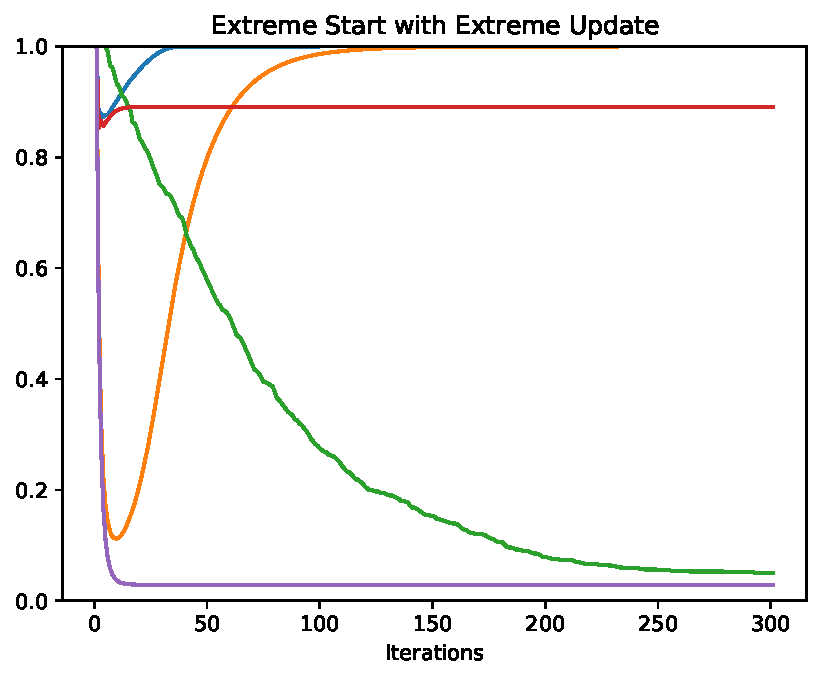
\includegraphics[width=\textwidth]{extremeextreme.pdf}
        \caption{SBM with half 1, -1 innate opinions.}
        \label{fig:extremeextreme}
    \end{subfigure}
    \begin{subfigure}[b]{0.4\textwidth}  
        \centering 
        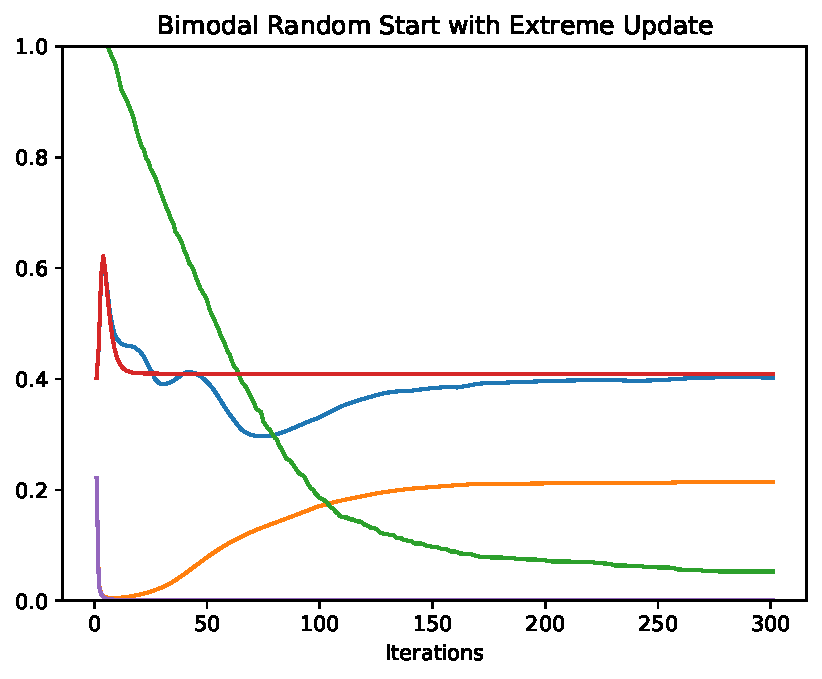
\includegraphics[width=\textwidth]{extremerandom.pdf}
        \caption{SBM with two scaled normal opinions.}
        \label{fig:extremerandom}
    \end{subfigure}
    \vskip\baselineskip
    \begin{subfigure}[b]{0.4\textwidth}   
        \centering 
        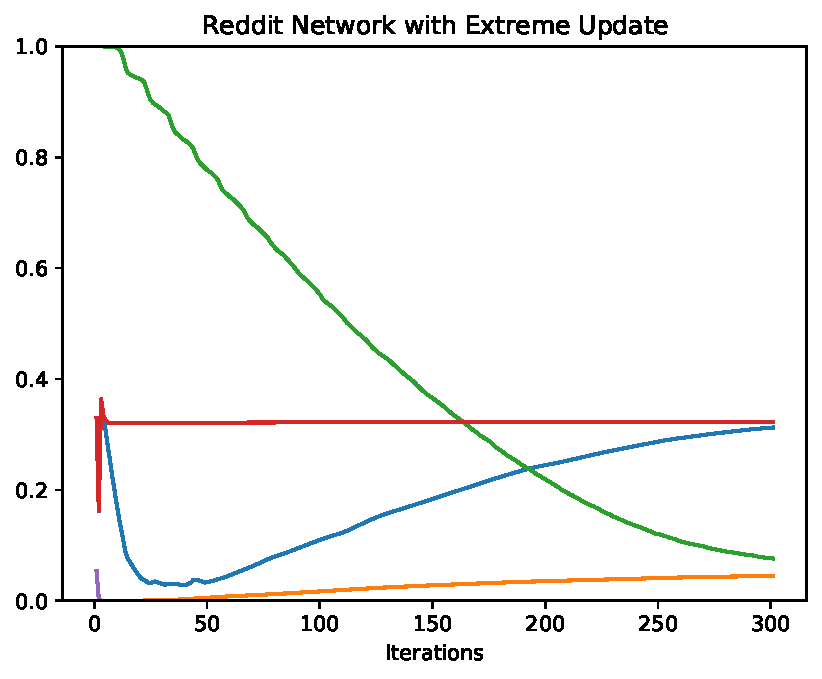
\includegraphics[width=\textwidth]{extremereddit.pdf}
        \caption{Posts on r/politics and other subreddits.}
        \label{fig:extremereddit}
    \end{subfigure}
    \begin{subfigure}[b]{0.4\textwidth}   
        \centering 
        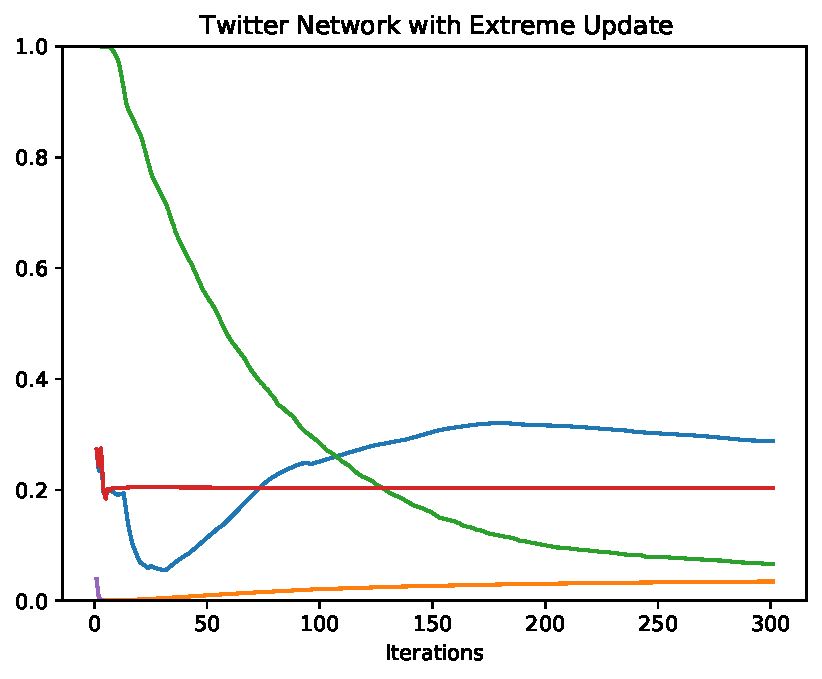
\includegraphics[width=\textwidth]{extremetwitter.pdf}
        \caption{2013 Delhi election opinions on Twitter.}
        \label{fig:extremetwitter}
    \end{subfigure}
    \caption{Difference between baseline and extreme administrator
    update on four different social network and opinion pairs.
    Brown corresponds to the ratio of remaining friendships in the baseline
    opinion formation process, green to friendships in the extreme update,
    red to bimodality in baseline, blue to bimodality in extreme,
    purple to polarization in baseline, and orange to polarization in extreme.}
    \label{fig:extreme}
\end{figure}

The extreme administrator update is a naive approach
to the natural mechanism social media platforms use
to boost engagement: increase exposure to content
similar in nature to user preferences
and simultaneously decrease exposure to content
dissimilar to user preferences.

While the overall weight (interpreted as time
by \cite{chitra20analyzing}) stays constant,
the individual level weight can move from one
node to another.
This combined with the elimination of friendships
suggest that the extreme update is not a reasonable
administrator action.
Nonetheless, analyzing it provides insight into an
intuitive idea and the extremes of a potential
administrator action.

\pagebreak

\subsection{Scaled Administrator Action}
The other administrator action we consider
is a less extreme variation.
Instead of subtracting weights from edges
and risking eliminating connections,
the scaled administrator only adds weights
and then normalizes to preserve the 
weights of each row.
The unfortunate result is that the
matrix is no longer symmetric.

\cref{lst:scaled} presents the pseudocode for
the scaled update.
The idea is that we want to add more weight
to edges close in opinion and less to edges far
in opinion.
We do this by taking 2 (the most extreme possible
difference between opinions) minus the absolute
difference in opinion for each node
and multiplying by $\epsilon$.
(Empirically, varying $0 \leq \epsilon \leq 1$
has a limited impact on the resulting figures.)
If two nodes have the same opinion, we add
$2\epsilon$; if their opinions are as far
apart as possible, we do not add any weight.

\begin{minipage}{\linewidth}
\begin{lstlisting}[caption={Scaled Administrator Update.}, label={lst:scaled}]
input: adjacency matrix $A$ of dimension $n\times n$,
        expressed opinions $z^{(t)}$,
        maximum edge change $\epsilon$ per iteration
output: modified adjacency matrix $A'$
$A' \gets$ copy of $A$
foreach $u$ in $[n]$ with more than one neighbor do
    $\Delta \gets \epsilon (A_{u,:} > 0)\times (2 - |z^{(t)}-z^{(t)}_u|)$ # resulting $\color{blue}n \times 1$ vector
    norm $\gets |\textrm{neighbors}|/(\sum_{v \in [n]}A_{u,v}+\Delta_v)$
    $A'_{u,:} \gets (A_{u,:}+\Delta)/$norm
return $A'$
\end{lstlisting}
\end{minipage}

\cref{fig:scale} shows bimodality and 
polarization as a function of iterations
for the baseline and scaled administrator update.
Notably, the time until the trends converge
is substantially smaller than the times
for the extreme update.

Across all four figures,
polarization reaches 0 fairly quickly.
The difference between the baseline and scaled update
is that the scaled bimodality is higher
most clearly in \cref{fig:scaletwitter}
but also in \cref{fig:scaleextreme}
and \cref{fig:scalereddit}.
Curiously, the bimodal SBM shows
no discernible difference between the baseline
and the scaled update.

\begin{figure}[h]
    \centering
    \begin{subfigure}[b]{0.4\textwidth}
        \centering
        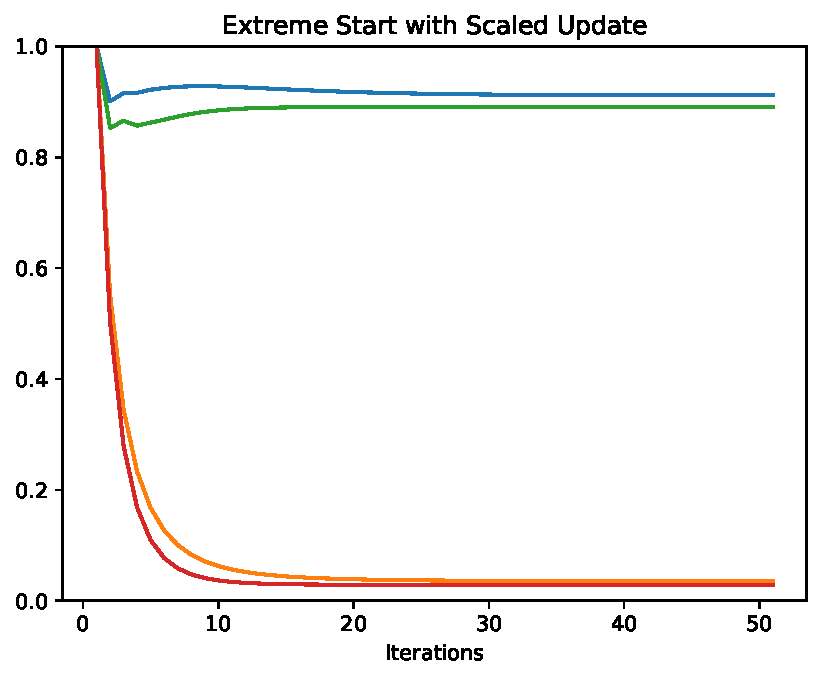
\includegraphics[width=\textwidth]{scaleextreme.pdf}
        \caption{SBM with half 1, -1 innate opinions.}
        \label{fig:scaleextreme}
    \end{subfigure}
    \begin{subfigure}[b]{0.4\textwidth}  
        \centering 
        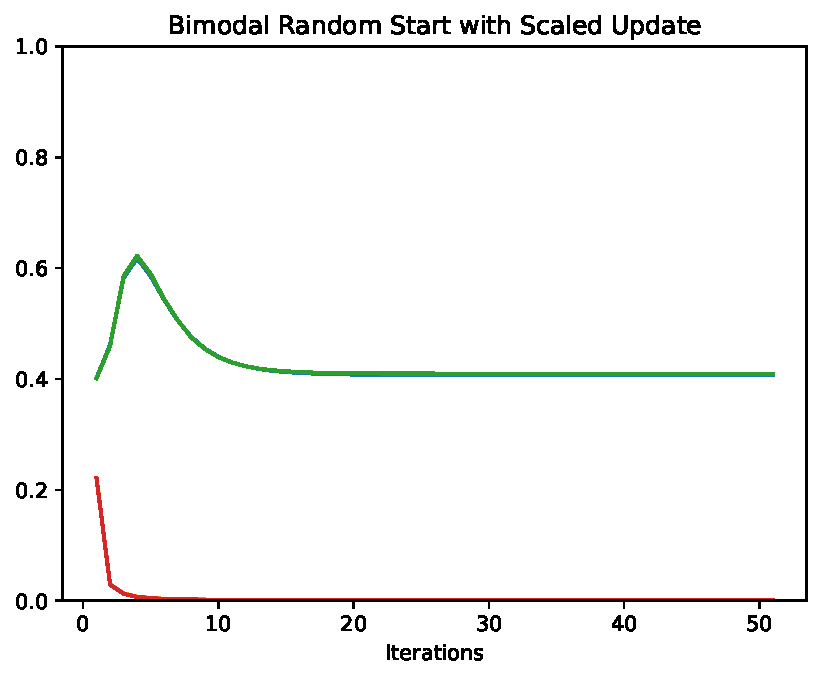
\includegraphics[width=\textwidth]{scalerandom.pdf}
        \caption{SBM with two normal opinions.}
        \label{fig:scalerandom}
    \end{subfigure}
    \vskip\baselineskip
    \begin{subfigure}[b]{0.4\textwidth}   
        \centering 
        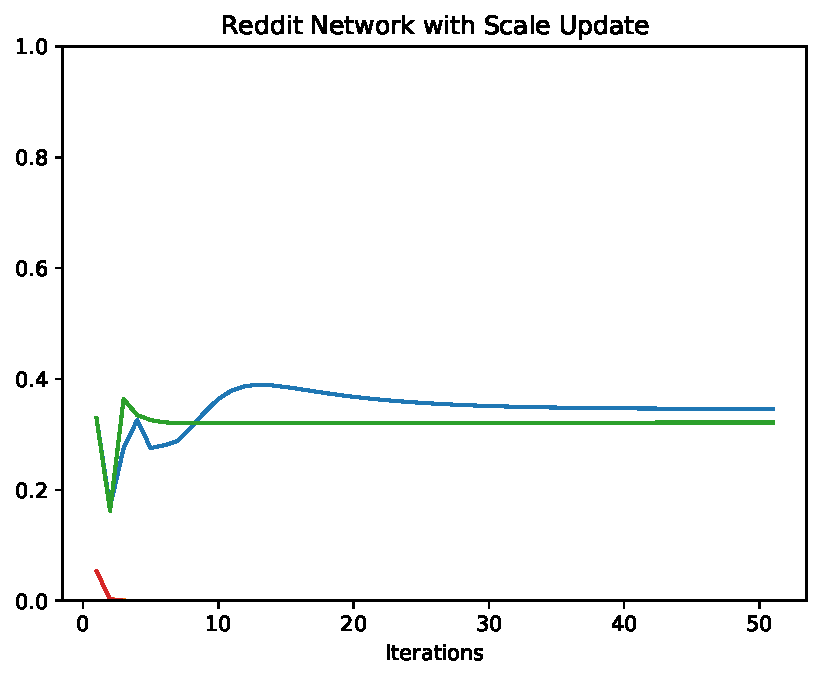
\includegraphics[width=\textwidth]{scalereddit.pdf}
        \caption{Posts on r/politics and other subreddits.}
        \label{fig:scalereddit}
    \end{subfigure}
    \begin{subfigure}[b]{0.4\textwidth}   
        \centering 
        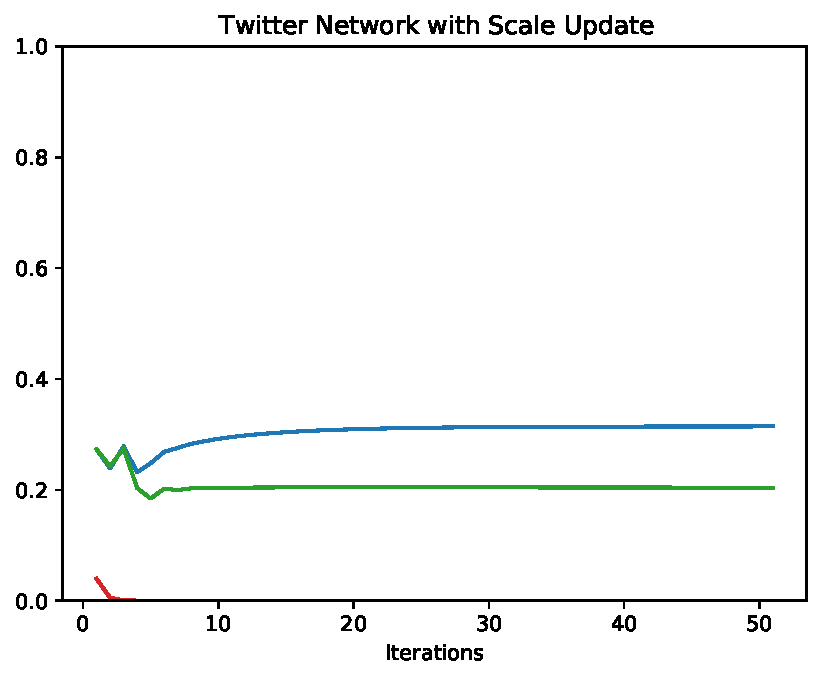
\includegraphics[width=\textwidth]{scaletwitter.pdf}
        \caption{2013 Delhi election opinions on Twitter.}
        \label{fig:scaletwitter}
    \end{subfigure}
    \caption{Difference between baseline and scaled administrator
    update on four different social network and opinion pairs.
    Green corresponds to bimodality in the baseline update,
    blue to bimodality in the scaled update,
    red to polarization in the baseline,
    and orange to polarization in the scaled update.}
    \label{fig:scale}
\end{figure}

The scaled update administrator action
takes a more subtle approach.
While the action boosts like-minded content,
the increase in bimodality is marginal
and the increase in polarization is negligible.

\subsection{Miscellaneous Variations}

In this section, we analyze the following variations and 
their effects on bimodality:
attacker nodes with an extreme opinion that do not update
their own opinion, three stochastic blocks rather than two,
and an imbalanced opinion (1/3-2/3 vs 1/2-1/2).

\begin{figure}[h]
    \centering
    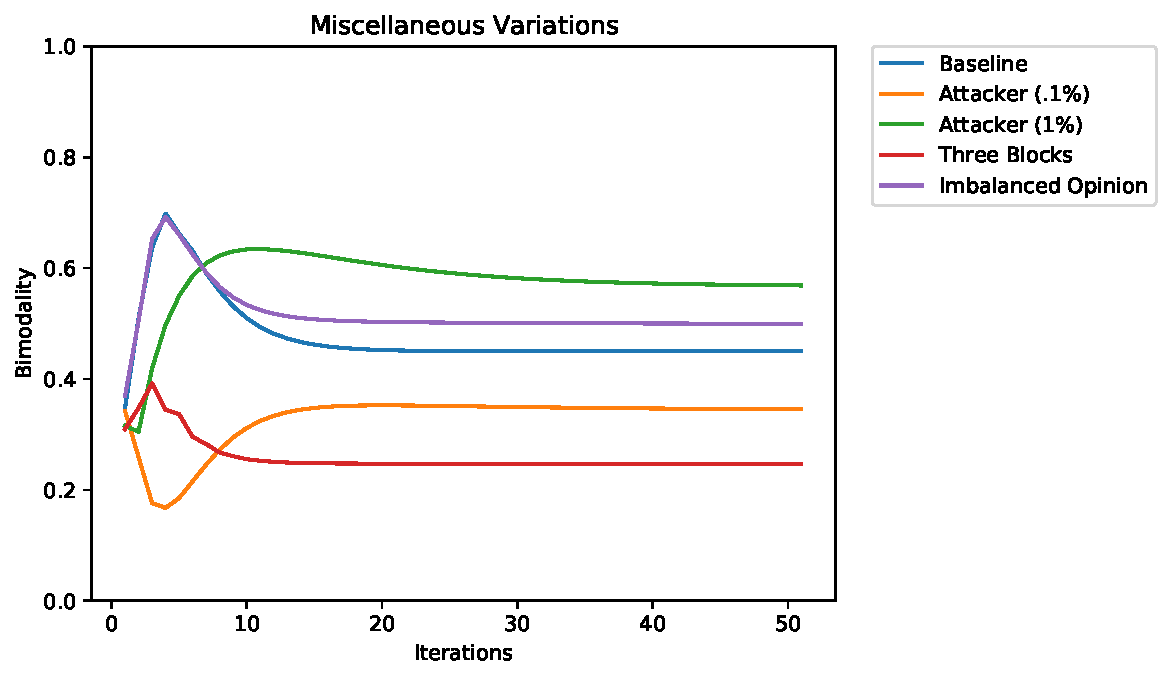
\includegraphics[width=.75\textwidth]{misc.pdf}
    \caption{SBM with half 1, -1 innate opinions.}
    \label{fig:misc}
\end{figure}

\autoref{fig:misc} shows the bimodality of each variation
on social networks with $n=1000$ nodes.
The imbalanced opinion is closest to the baseline,
maintaining essentially the same bimodality until the $10$th
iteration when the bimodality of the imbalanced opinion increases.
The attacker node that constitutes .1\% of the population
ironically seems to reduce bimodality.
The attacker nodes that constitute 1\% of the population
markedly increase bimodality as we would expect.
Finally, the three block model has the lowest bimodality.
This makes sense given that the three blocks are centered
at .5, 0, -.5 respectively rather than the more polarized
.5 and -.5.

